\section{Development Workflow}

We motivate our development workflow from previous work 
\cite{PureScript2019} by extending the \fancyname{Scribble} toolchain
and generating APIs that integrate the developer's 
application logic
into the execution of the communication automata.

We visualise the workflow in \cref{fig:devworkflow} 
and provide a brief overview:

\begin{enumerate}

\item The developer supplies the communication protocol written in
\fancyname{Scribble} (\cref{subsection:scribble}), 
stating the role (hereafter \textit{endpoint})
to generate APIs for,
and the code generation \textit{target} 
(i.e. whether the role runs on the server or the web browser).

\item \fancyname{SessionTS} delegates to the 
\fancyname{Scribble} toolchain for verifying the well-formedness of
the protocol and expects to receive a DOT graph representation of
the endpoint FSM (\cref{subsection:efsm}). 
\fancyname{SessionTS} parses the endpoint's 
interactions from the DOT graph and generates TypeScript APIs
for the developer (\cref{subsection:apigen}) 
tailored to the specified target.

\item The developer implements their web application using the
generated APIs. Implementations that pass the type-checking phase
of the TypeScript Compiler are guaranteed to be free from 
communication errors by session type theory.

\end{enumerate}

\begin{figure}[!ht]
\centering
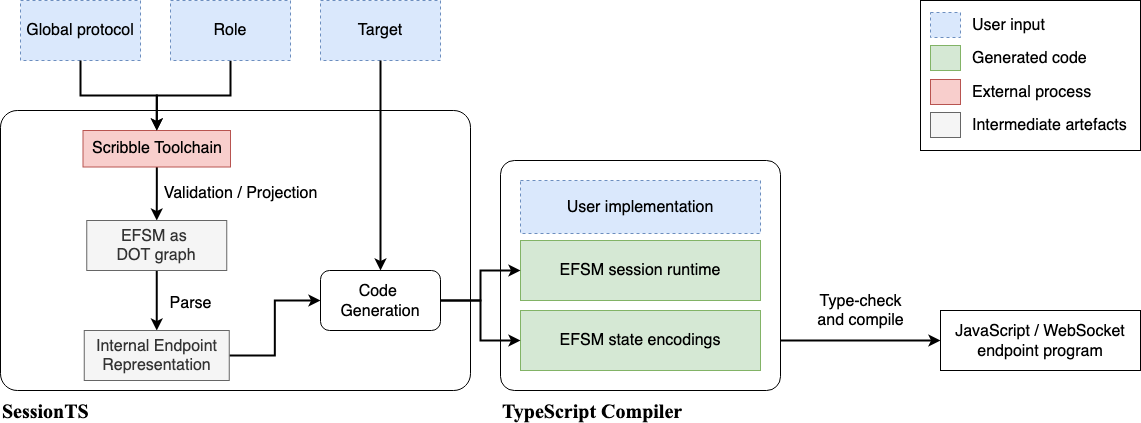
\includegraphics[width=\textwidth]{DevelopmentWorkflow}
\captionof{figure}{Overview of \fancyname{SessionTS} Development Workflow}
\label{fig:devworkflow}
\end{figure}

\subsection{Protocol Specification with \fancyname{Scribble}}
\label{subsection:scribble}

We use the \fancyname{Scribble} protocol description language, 
as presented in
\cite{Scribble}, for formalising the communication structure. This is
inspired by existing work on implementing session type theory 
in mainstream programming languages
\cite{Hybrid2016, PureScript2019, Python2017}. 
We use the variant of the \fancyname{Scribble} language 
previously introduced in \cref{subsection:bgscribble}.

\subparagraph{Type declaration statements}
Specific to our TypeScript API generation toolchain,
the developer is \textit{not} required to explicitly
add type declaration statements for built-in types.
\cref{lst:adder} is a \textit{syntactically correct}
\fancyname{Scribble} protocol as far as 
\fancyname{SessionTS} is concerned. 
Internally, \fancyname{SessionTS} inspects the protocol file
and parses existing type declarations using regular expressions
(or \textit{regex}) -- this is necessary to extract any
custom data types that will appear in the communication (for example,
\cref{lst:game}), and allows \fancyname{SessionTS} to inject
``boilerplate'' type declarations for built-in TypeScript types before
calling \fancyname{Scribble}.

\begin{figure}[!ht]
\begin{lstlisting}[language=Scribble]
module Adder;

global protocol Adder(role Client, role Svr) {
	choice at Client {
		ADD(number, number) from Client to Svr;
		RES(number)         from Svr to Client;	
	} or {
		QUIT(string) from Client to Svr;	
		TERMINATE()  from Svr to Client;
	}
}
\end{lstlisting}
\captionof{lstlisting}{The \tprotocol{Adder} Protocol}
\label{lst:adder}
\end{figure}

We will use the \tprotocol{Adder} protocol as a running example
to demonstrate how our work performs TypeScript API generation.

\subsection{From \fancyname{Scribble} to EFSM}
\label{subsection:efsm}

Given the protocol and endpoint, we use \fancyname{Scribble}
to validate the well-formedness of the protocol and extract
information from the protocol relevant for the endpoint.
The latter is expressed as a finite state machine
where each state restricts the possible transitions, 
and transitions between states are represented by
communication actions, i.e. the sending or receiving of a message.

\fancyname{Scribble} expresses the EFSM using the 
DOT graph description language \cite{dot}, with each
communication action encoded as the label of the corresponding
state transition. 
\fancyname{SessionTS} uses the pydot library \cite{pydot}
to parse the graph into an internal representation of the EFSM.
We define an \texttt{EfsmBuilder} class with APIs designed for
constructing the EFSM representation by iterating over the 
state transitions from the DOT representation.

\begin{figure}[!ht]
\begin{lstlisting}[language=Python]
@dataclass
class Endpoint:
    protocol: str
    role    : str
    server  : str
    efsm    : EFSM
    types   : typing.Iterable[DataType]
\end{lstlisting}
\captionof{lstlisting}{The Endpoint API}
\label{lst:endpointapi}
\end{figure}

As the code generation process requires additional information,
we define an \texttt{Endpoint} dataclass\footnote{
A Python dataclass uses the decorator to generate
``boilerplate'' methods, such as the constructor, based on the
properties listed in the annotations.} (\cref{lst:endpointapi})
to contain the \texttt{EFSM}
representation, along with the information passed in from the
command line (\texttt{protocol}, \texttt{role}, \texttt{server}) 
and the custom type declarations (\texttt{types}) parsed from the
protocol specification.

\subsection{API Generation}
\label{subsection:apigen}

Formally, API generation is a function of the constructed
\texttt{Endpoint} instance
\textit{and} the target specified in the command line. We use a 
different code generation strategy for implementations running on
Node.js versus the browser -- we discuss in greater depth in 
\cref{chap:node} and \cref{chap:react} respectively. 
In this subsection, we explain how we perform API generation
at a higher level of abstraction.

Traditional methods of code generation involve applying the
Visitor pattern on the internal representation. 
In the context of the MPST framework,
this may involve defining a Visitor class that implements a
\texttt{generate()} operation to be performed on the EFSM states,
such that the \texttt{generate()} implementation specialises to the
type of EFSM state, i.e. send, receive or terminal.
This is not straightforward in Python, as method overloading is not 
supported, so the ``visit'' methods would need different names.
More importantly, it is less straightforward to visualise
the structure of the generated code, as the string interpolation
aspect is likely to be interleaved with source code implementing
additional logic for code generation.

For \fancyname{SessionTS}, we opt to use a template engine for code
generation, namely Jinja \cite{jinja}.

\dots %what is a template, 
\dots %template focuses on how the generated code looks (which makes it easy to debug etc), and uses lightweight markup syntax to inject dynamic content (from our endpoint API)

The main advantage of using a template engine for 
our code generation task is that it decouples the ``presentation''
from the ``content'': in the \fancyname{SessionTS}
% so it is easy to prototype and extend without touching the source code

\begin{itemize}
\item api generation is a function of the EFSM representation
\item traditional methods -- visitor pattern on the EFSM and using stringbuilder to build the file
\item templating library is more suitable to decouple the ``presentation'' (how the code should look) from the ``content'' (the EFSM which is used to build the code)
\item strategy pattern to support the two required build targets (in node and react)
\end{itemize}